\documentclass[10pt,conference]{IEEEtran}
\IEEEoverridecommandlockouts

\usepackage{cite}
\usepackage{amsmath,amssymb,amsfonts}
\usepackage{graphicx}
\usepackage{textcomp}
\usepackage{xcolor}
\usepackage{booktabs}
\usepackage{multirow}
\usepackage{array}

\begin{document}

\title{Beyond Self-Assessment: Iterative Safety Refinement with External Security Signals}

\author{}
\maketitle

\begin{abstract}
Large Language Models (LLMs) frequently generate code that is functionally correct yet harbors memory-safety vulnerabilities. Existing approaches to safe code generation---prompt engineering, constrained decoding, and LLM self-repair---share a common limitation: they ultimately rely on the LLM's own ability to assess and reason about code security, a capability our experiments show to be unreliable. We present Iterative Safety Refinement (ISR), a framework that decouples safety assessment from generation by introducing an independently trained, frozen security classifier as an external feedback signal. In each iteration, the LLM generates code, the classifier scores it and identifies attention-weighted vulnerable tokens, and targeted feedback guides repair. We benchmark ISR against four baselines spanning prompt engineering, prefix steering, and LLM self-reflection across nine method configurations (ISR variants + four baselines), generating and automatically evaluating thousands of code samples. A unified human evaluation of 320 LLM-generated C functions across 15 memory-safety-critical tasks and three independently evaluated LLMs confirms the classifier-based ranking is unreliable and serves as the primary comparison. ISR achieves an \textbf{87.5\%} human-evaluated safety rate, surpassing the strongest baseline by 4.2 percentage points and improving over the no-feedback lower bound by \textbf{42 percentage points}, while preserving functional correctness on all 21 test cases. ISR's effectiveness generalizes across three independently evaluated LLMs, with consistent safety gains of 40--54 percentage points. Ablation experiments reveal a monotonic relationship between feedback precision and human-evaluated safety: each level of refinement---from generic alerts (ISR-1) to attention-guided localization (ISR-2) to specification-augmented feedback (ISR-3)---yields consistent gains across all three models. Precise localization enables a four-order-of-magnitude P(vul) reduction (0.806 $\rightarrow$ 0.000070), while the classifier perspective alone is misleading, as ISR-3's human safety rate is the highest despite sub-optimal classifier scores. Further analysis exposes a cross-domain distribution shift: the classifier, despite attaining F1=0.896 on its MSR training distribution, exhibits near-zero correlation with human safety judgments on LLM-generated code (Spearman's $\rho$=0.04), causing all baseline safety rates to be overestimated by 10--15 percentage points. ISR remains effective despite this imperfect signal, demonstrating that external feedback mechanisms offer a viable path toward safe LLM code generation.
\end{abstract}

\begin{IEEEkeywords}
LLM code generation, memory safety, iterative safety refinement, security classifier, cross-domain distribution shift
\end{IEEEkeywords}

\section{Introduction}

Large Language Models have demonstrated remarkable capability in code generation, powering tools used by millions of developers. However, a critical tension persists: LLM-generated code often achieves functional correctness while harboring memory-safety vulnerabilities such as buffer overflows, use-after-free errors, and null pointer dereferences. Recent empirical studies reveal the scale of this problem: 27.3\% of Copilot-generated code contains security vulnerabilities~\cite{copilotsec}, LLM-based code generation exhibits vulnerability rates of 18--50\% across different models and scenarios~\cite{chromesecbench}, and existing safety mechanisms are easily bypassed---CodeAttack achieves over 80\% success in circumventing LLM safety guards via code inputs~\cite{codeattack}, while CodeJailbreaker reaches 94.35\% attack success rate by hiding malicious intent in commit messages~\cite{codejailbreaker}. In practice, the same prompt can elicit safe code from one model and vulnerable code from another---Opus generates parameterized queries while Sonnet produces SQL injection patterns under identical task descriptions. This inconsistency reveals a fundamental problem: \textit{LLMs lack reliable mechanisms to assess the security properties of their own generated code}.

Existing approaches to safe code generation fall into three categories. \textbf{Static analysis tools} (e.g., Flawfinder) operate on completed code but cannot distinguish functionally equivalent code blocks with different safety properties. \textbf{Prompt engineering methods} such as SVEN~\cite{sven} and SafePrompt enrich prompts with security prefixes or specifications, but plateau in effectiveness and rely on the LLM's own (unreliable) interpretation of safety constraints. \textbf{LLM self-assessment methods} such as Reflexion~\cite{reflexion} and CoSec~\cite{cosec} let the LLM review its own output and self-correct---but our experiments reveal this self-assessment is no better than random, and self-correction degrades code more often than it improves it (10/15 cases for Reflexion).

A deeper issue underlies these failures. Recent research has established that more capable reasoning does not imply safer output: long Chain-of-Thought (CoT) reasoning~\cite{cot} does not guarantee safety~\cite{safechain}, self-consistency mechanisms are vulnerable to systematic errors~\cite{tooconsistent}, and even CoT safety monitoring is fragile~\cite{cotmonitor}. In fact, stronger reasoning models can perform \textit{worse} on security~\cite{chromesecbench,lrmsafety}. All three existing paradigms for safe code generation share a common root cause: they depend on the LLM's own ability to reason about code security. We argue that this is circular---the same model that generated vulnerable code cannot be trusted to reliably assess whether that code is safe. An external, objective safety signal is needed.

We propose \textsc{SecurePath}, a framework that decouples safety assessment from code generation. The key insight is simple: an independently trained security classifier can provide an external signal that guides iterative code refinement, even if that signal is imperfect. Our approach consists of two stages:

\begin{enumerate}
\item \textbf{Security-aware training}: A CodeBERT-based encoder trained with contrastive learning on carefully constructed vulnerability/safety pairs (solution two preprocessing), followed by an AttentionPooling-based safety classifier (F1=0.896, AUC=0.953 on MSR test data).
\item \textbf{Iterative Safety Refinement (ISR)}: Code generation $\rightarrow$ classifier scoring $\rightarrow$ targeted feedback $\rightarrow$ repair, iterated until convergence or maximum rounds.
\end{enumerate}

We evaluate \textsc{SecurePath} against four baselines spanning prompt engineering, prefix steering, and LLM self-reflection on a unified human evaluation benchmark totaling 320 code samples across 15 memory-safety-critical prompts and three independently evaluated LLMs. Our results reveal:

\begin{itemize}
\item \textbf{ISR outperforms all baselines}: ISR-3 achieves 87.5\% human-judged safety rate, surpassing SafePrompt (71.4\%), CoSec (76.7\%), SVEN (78.6\%), and Reflexion (83.3\%).
\item \textbf{Feedback precision drives monotonic safety improvement}: Human-evaluated safety rate increases with each level of feedback precision---generic $\rightarrow$ attention-guided $\rightarrow$ specification-augmented---across all three models. Precise localization enables a headline case of 0.806 $\rightarrow$ 0.000070 P(vul) reduction, and the security specification provides an additional +6.7--7.5pp human safety gain beyond attention alone.
\item \textbf{A critical cross-domain finding}: The classifier's P(vul) scores show near-zero correlation with human safety judgments on LLM-generated code (Spearman's $\rho=0.04$ on DeepSeek-v4-pro, $\rho \leq 0.27$ across three LLMs), and the safety rates reported by all baselines are inflated by 10--15 percentage points compared to human assessment.
\item \textbf{ISR works despite imperfect signals}: Even with $\rho=0.04$, iterative refinement improves the human safety rate from 45.5\% (no feedback) to 87.5\%.
\end{itemize}

Our work makes three contributions: (1) we propose and validate ISR, a practical framework for LLM code safety that outperforms representative baselines on unified human evaluation while preserving functional correctness (21/21 test cases passed); (2) we provide the first empirical evidence of MSR-to-LLM domain shift in code security classification, and demonstrate that it leads to systematic overestimation of baseline safety rates; (3) we show that external feedback mechanisms remain effective even when the signal itself is imperfect, suggesting a path forward for safe LLM-based code generation.

\section{Related Work}

\subsection{Vulnerability Detection}

Deep learning has been widely applied to source code vulnerability detection. Approaches range from graph-based representations (Devign~\cite{devign}, SySeVR~\cite{sysevr}) leveraging CPG and AST structure, to sequence-based models (LineVul~\cite{linevul}, VulDeePecker~\cite{vuldeepecker}) operating on code tokens. CodeBERT~\cite{codebert} and GraphCodeBERT~\cite{graphcodebert} provide pre-trained representations that capture both syntactic and semantic code properties. A comprehensive survey~\cite{vuldetectionsurvey,llmsecuritysurvey} documents the evolution from pattern matching to deep learning for vulnerability discovery, though data quality and label accuracy remain persistent concerns~\cite{primevul}.

These methods achieve strong performance on curated datasets (e.g., MSR, BigVul, Devign) but operate under a critical assumption: that the training and deployment distributions match. Our work demonstrates that this assumption breaks when applying MSR-trained classifiers to LLM-generated code---the domain shift is severe enough to render the classifier signal essentially unusable for evaluating LLM-generated code (Spearman's $\rho=0.04$). To our knowledge, this is the first empirical characterization of MSR-to-LLM domain shift in code security.

\subsection{Safe Code Generation}

\textbf{Prompt-based steering.} SVEN~\cite{sven} (CCS 2023) proposes prefix-guided safety steering, where a learned continuous prefix is prepended to the LLM prompt to bias generation toward safer completions. SafePrompt enriches task descriptions with explicit safety requirements (bound checking, null validation, safe string operations). These methods improve safety but ultimately depend on the LLM's interpretation of safety constraints---they cannot verify whether the generated code actually satisfies them.

\textbf{Security co-decoding.} CoSec~\cite{cosec} (ISSTA 2024) decomposes generation into two phases: first producing a security specification, then generating code with inline security annotations. While this approach provides more explicit safety guidance, our experiments show that its built-in self-audit mechanism provides no meaningful discrimination (nearly all candidates rated as fully safe regardless of actual vulnerability).

\textbf{Constrained and mechanistic approaches.} Constrained decoding~\cite{constraineddecode} enforces security rules at the token level during generation, preventing unsafe function calls and patterns. THEA~\cite{thea} (ICSE 2026) uses sparse autoencoders to identify and manipulate safety-relevant internal representations within the LLM during inference, achieving a 15\% improvement on CyberSecEval. These methods are effective but require white-box access to model internals or decoding procedures, limiting applicability to proprietary API-based models.

\textbf{LLM self-reflection and repair.} Reflexion~\cite{reflexion} (NeurIPS 2023) introduces a self-review-and-repair loop where the LLM audits its own code for security issues, then regenerates. We replicate this approach and find that while the best iteration is often the initial generation, the self-reflection mechanism degrades safety in 10/15 cases. SecRepair~\cite{secrepair} augments LLM-based repair with reinforcement learning and semantic rewards, but similarly relies on the LLM's own vulnerability identification capability. Complementary directions include multi-agent deliberation for safety reasoning data~\cite{aidsafe} and VICS-guided prompting for vulnerability data generation~\cite{vics}.

CodeSecEval~\cite{codesec} establishes a benchmark of 44 vulnerability types for evaluating LLM code security, while H-CoT~\cite{hcot} demonstrates that CoT safety mechanisms can be hijacked to reduce refusal rates from 98\% to below 2\%.

\textbf{Fundamental limitation.} All existing safe generation methods rely on the LLM's own understanding of code security, whether through prompt interpretation, self-generated specifications, or self-audit. \textsc{SecurePath} differs fundamentally: the safety signal comes from an independently trained, frozen classifier. This external signal is imperfect---as we demonstrate---but even an imperfect external signal outperforms the LLM's self-assessment.

\textbf{The evaluation problem.} A recent study~\cite{rethinking} (ICSE 2026) systematically demonstrates that existing security guard methods for code LLMs achieve their reported gains primarily by trading off functional correctness---the guarded models produce safer but functionally broken code. This finding fundamentally challenges the evaluation methodology of prior work and motivates us to explicitly verify functional correctness preservation in \textsc{SecurePath} (Section~\ref{sec:functional}).

\subsection{Contrastive Learning and Code Representation}

InfoNCE-based contrastive learning~\cite{infonce} has been successfully applied to code representation learning, enabling models to distinguish semantically similar from dissimilar code fragments. SimCSE~\cite{simcse} (EMNLP 2021) demonstrates that simple contrastive learning with dropout-based augmentation produces high-quality sentence embeddings. We adopt this paradigm in our encoder pre-training stage, with careful data construction (solution two) to ensure meaningful contrastive pairs. Prototypical Networks~\cite{protonet} (NeurIPS 2017) formalize class representations as the mean of support set embeddings---we leverage this concept in our prototype-based ablation, finding that binary cosine-threshold classification fails to capture the non-linear boundary between safe and vulnerable code.

\subsection{Reasoning Path Selection and Self-Consistency}

Our ISR framework iteratively selects and refines code across multiple generation rounds, connecting to a broader literature on reasoning path selection. The foundational Self-Consistency method~\cite{selfconsistency} (ICLR 2023) improves CoT reasoning by sampling multiple paths and taking a majority vote. However, subsequent work reveals critical limitations: self-consistent errors---where the model confidently produces the same wrong answer across samples---are difficult to detect and increase with model scale~\cite{tooconsistent} (EMNLP 2025).

Several improvements have been proposed, including confidence-weighted voting~\cite{cisc} and continuous likelihood scoring~\cite{softsc}, though none address the fundamental issue of selection criterion quality: rather than selecting paths by confidence, consistency, or likelihood, we select by \textit{external safety signal}. The finding that self-consistency is fragile~\cite{tooconsistent} and that stronger reasoning does not guarantee safety~\cite{safechain,lrmsafety} directly motivates our departure from internal selection criteria.

\section{Method}

\begin{figure*}[t]
\centering
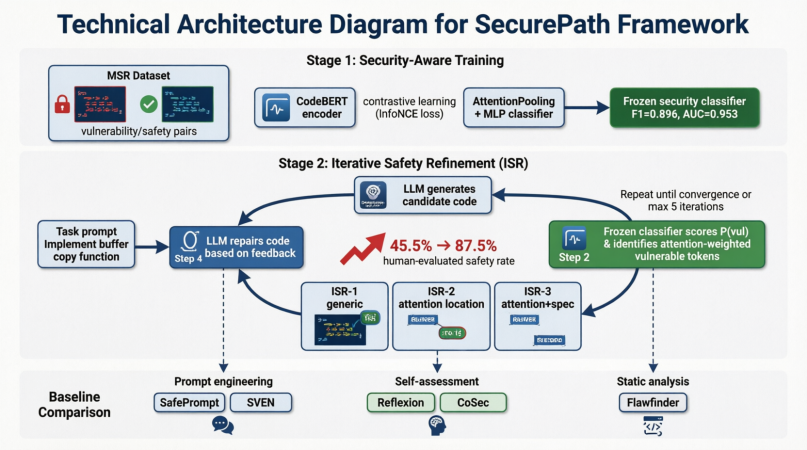
\includegraphics[width=\textwidth]{fig/1.png}
\caption{Overview of the \textsc{SecurePath} framework. Stage 1: A CodeBERT-based encoder is trained with contrastive learning on safety/vulnerability pairs. Stage 2: An AttentionPooling classifier is trained on the frozen encoder. Stage 3: ISR iteratively refines LLM-generated code using classifier feedback---scoring, attention-weighted token localization, and targeted repair.}
\label{fig:framework}
\end{figure*}

Our approach, illustrated in Figure~\ref{fig:framework}, consists of two training stages followed by an iterative refinement procedure at inference time.

\subsection{Data Preprocessing: Solution Two}

A critical but often overlooked issue in vulnerability dataset construction is the semantic equivalence of positive and negative samples. In the MSR dataset, records with \texttt{vul=0} (safe code) have identical \texttt{func\_before} and \texttt{func\_after} in 92.7\% of cases---the function was already safe and required no fix. Naively mixing \texttt{vul=0} records with \texttt{vul=1} records for contrastive learning causes feature collapse, as the model is forced to learn that ``identical code is both safe and vulnerable.'' We observed accuracy dropping to 52\% under this naive approach.

\textbf{Solution two} constructs separate pools:
\begin{itemize}
\item \textbf{Vulnerability pool}: \texttt{vul=1} $\rightarrow$ \texttt{func\_before} (7,901 functions).
\item \textbf{Safety pool}: \texttt{vul=0} $\rightarrow$ \texttt{func\_before} (111,087) + \texttt{vul=1} $\rightarrow$ \texttt{func\_after} (7,901).
\end{itemize}
This ensures that vulnerability and safety code come from \textit{different functions}, creating genuine semantic distinctions. From these pools, we sample 5,498 training pairs (2,749 vul + 2,749 safe) balanced across six CWE types (CWE-119, 125, 190, 416, 476, 787).

\subsection{Stage 1: Security-Aware Encoder}

We fine-tune CodeBERT-base (125M parameters) with contrastive learning using InfoNCE loss~\cite{infonce}, following the SimCSE~\cite{simcse} paradigm of dropout-based augmentation for robust representation learning. The encoder learns to map vulnerable and safe code into well-separated regions of a shared embedding space. On a held-out pair matching task, the encoder achieves 85.7\% accuracy in distinguishing vulnerability/safety pairs from random pairings.

\subsection{Stage 2: Safety Classifier}

The classifier uses a frozen CodeBERT encoder followed by an AttentionPooling layer (rather than CLS pooling) and a three-layer MLP (768 $\rightarrow$ 256 $\rightarrow$ 128 $\rightarrow$ 2). Total trainable parameters: $\sim$820K (590K attention + 230K MLP).

\begin{table}[h]
\centering
\caption{Classifier architecture comparison on MSR test set.}
\begin{tabular}{lccc}
\toprule
Architecture & F1 & AUC & Params \\
\midrule
CLS Pooling & 0.884 & 0.949 & $\sim$230K \\
\textbf{AttentionPooling} & \textbf{0.896} & \textbf{0.953} & $\sim$820K \\
\bottomrule
\end{tabular}
\end{table}

A prototype-based ablation---using cosine similarity to vulnerability/safety centroids \`{a} la Prototypical Networks~\cite{protonet}---achieves only F1=0.67 (binary thresholding fails, always predicting ``vulnerable''), confirming that a non-linear decision boundary with token-level attention is necessary.

Cross-CWE leave-one-out evaluation demonstrates strong generalization: average F1=0.8944 across all held-out CWE types, only 0.0015 below the full-training F1, indicating the classifier learns generic safety patterns rather than CWE-specific shortcuts.

\subsection{Iterative Safety Refinement (ISR)}

ISR operates through a simple loop:

\begin{enumerate}
\item \textbf{Generate}: LLM produces candidate code for a given task prompt.
\item \textbf{Score}: The frozen safety classifier computes P(vul) and, for ISR-2/3, identifies attention-weighted vulnerable tokens.
\item \textbf{Feedback}: A feedback prompt is constructed based on the ablation setting (generic / attention location / location + security specification).
\item \textbf{Repair}: The LLM regenerates the code based on the feedback.
\item \textbf{Repeat}: Steps 2--4 iterate until P(vul) stops improving (stagnation) or max 5 iterations.
\end{enumerate}

We design five ablation configurations to isolate the contribution of feedback precision:

\begin{table*}
\centering
\caption{ISR ablation configurations.}
\begin{tabular}{lccccp{3.5cm}}
\toprule
Config & Feedback & Generic & Attention & Spec & Research Question \\
\midrule
ISR-0 & $\times$ & $\times$ & $\times$ & $\times$ & Single-generation lower bound \\
ISR-1 & $\checkmark$ & $\checkmark$ & $\times$ & $\times$ & Is vague feedback enough? \\
ISR-2 & $\checkmark$ & $\times$ & $\checkmark$ & $\times$ & Precise localization, no instruction \\
ISR-random & $\checkmark$ & $\times$ & rnd & $\times$ & Is attention localization causal? \\
ISR-3 & $\checkmark$ & $\times$ & $\checkmark$ & $\checkmark$ & Full: localization + safety spec \\
\bottomrule
\end{tabular}
\end{table*}

\textbf{ISR-1} (Generic): ``This code has security issues. Please fix them.''---tests whether the mere presence of an external alert improves safety.

\textbf{ISR-2} (Attention): ``Line X, [specific token pattern] is unsafe. Please fix it.''---provides precise location but does not prescribe \textit{how} to fix.

\textbf{ISR-random} (Random Attention): Identical to ISR-2 in every respect except one: the code regions flagged as ``high attention'' are randomly sampled from syntactically valid code spans, rather than drawn from the classifier's actual attention weights. The feedback format, iteration protocol, and stopping criteria are identical to ISR-2. This ablation directly tests whether the classifier's \textit{spatial localization} signal is causal---if attention-guided feedback works better than randomly pointing at code, the classifier's token-level signal must carry genuine information beyond what generic iteration provides.

\textbf{ISR-3} (Attention+Spec): ``Line X, [pattern] is unsafe. A safe implementation must: validate all inputs before use, check buffer bounds for every write, handle NULL pointers explicitly, and avoid unsafe standard library functions.''---provides both precise location and normative safety guidance.

\section{Experiments}

\subsection{Experimental Setup}

\textbf{Training data}: MSR\_data\_cleaned, 188,636 functions across 6 CWE types. After solution two preprocessing: 3,375 training / 482 validation / 965 test.

\textbf{Models}: CodeBERT-base (125M, frozen) for encoding. DeepSeek-v4-pro for primary code generation experiments (temperature=0.8). Cross-model validation uses GLM-5.1 and Sonnet-4-6 under the same protocol.

\textbf{Evaluation prompts}: 15 memory-safety-critical C programming tasks, covering buffer operations (P01, P09, P10, P13), memory management (P03, P05, P11, P12, P14), pointer safety (P02, P04, P08), I/O handling (P06), input parsing (P07, P15).

\textbf{Human evaluation}: 320 code samples in total (80 for DeepSeek-v4-pro primary evaluation, 120 each for GLM-5.1 and Sonnet-4-6 cross-model validation), stratified by P(vul) band and method source, blinded (evaluator sees only the prompt description and code). Binary judgment: SAFE (no memory-safety vulnerability) or UNSAFE (at least one confirmed issue).

\textbf{Baselines}: SafePrompt (B4), SVEN (B5, CCS 2023), Reflexion (B6, NeurIPS 2023), CoSec (B7, ISSTA 2024). All generate 10 candidates per prompt and select the one with the lowest classifier P(vul).

\subsection{Classifier Performance on MSR Domain}

On the in-domain MSR test set, the AttentionPooling classifier achieves F1=0.896 and AUC=0.953. Per-CWE analysis shows consistent performance across all six vulnerability types (F1 range: 0.887--0.938). Leave-one-out cross-CWE generalization yields an average F1 of 0.8944, only 0.0015 below the full-training baseline, confirming the model learns generic safety representations rather than CWE-specific shortcuts.

\subsection{ISR vs. Baselines: Unified Human Evaluation}

Table~\ref{tab:unified} presents the core result on DeepSeek-v4-pro: all methods evaluated on the same 80 code samples by the same human evaluator using the same criteria.

\begin{table*}
\centering
\caption{Unified human evaluation comparison on DeepSeek-v4-pro. All methods evaluated on identical prompts and criteria.}
\label{tab:unified}
\begin{tabular}{lccp{4cm}}
\toprule
Method & Human SAFE Rate & Type & Mechanism \\
\midrule
ISR-0 (no feedback) & 45.5\% & Lower bound & Single generation \\
ISR-1 (generic) & 72.7\% & ISR ablation & Vague safety feedback \\
SafePrompt (B4) & 71.4\% & Prompt engineering & Safety-enhanced prompt \\
CoSec (B7, ISSTA 2024) & 76.7\% & Academic baseline & Security spec + self-audit \\
SVEN (B5, CCS 2023) & 78.6\% & Academic baseline & Prefix-guided steering \\
ISR-2 (attention) & 80.0\% & ISR ablation & Precise location feedback \\
Reflexion (B6, NeurIPS 2023) & 83.3\% & Academic baseline & LLM self-review + repair \\
\textbf{ISR-3 (attention+spec)} & \textbf{87.5\%} & \textbf{Our method} & \textbf{Precise feedback + spec} \\
\bottomrule
\end{tabular}
\end{table*}

\textbf{Key findings:}

\textit{ISR-3 achieves the highest human-evaluated safety rate} (87.5\%), exceeding the strongest baseline (Reflexion, 83.3\%) by 4.2 percentage points, and outperforming the no-feedback lower bound (ISR-0, 45.5\%) by 42 percentage points.

\textit{External feedback monotonically improves safety.} ISR-0 (45.5\%) $\rightarrow$ ISR-1 (72.7\%) $\rightarrow$ ISR-2 (80.0\%) $\rightarrow$ ISR-3 (87.5\%), a monotonic trend with increasing feedback precision. Each step from no feedback to generic to attention-based to specification-enriched feedback yields a meaningful safety gain.

\textit{Prompt engineering and self-assessment methods fall short.} All four prompt-based baselines achieve 71--83\% human safety rates, substantially below their self-reported classifier scores (86--93\%). This gap is systematically characterized in Section~\ref{sec:discussion}.

\textbf{P01\_buffer\_copy: a common blind spot on DeepSeek-v4-pro.} All four baselines fail to produce a safe buffer copy implementation under any configuration---a task that ISR-3 handles correctly. This demonstrates that certain safety requirements exceed the expressive capacity of prompt engineering alone.

\subsection{ISR Ablation: Classifier Perspective}

Table~\ref{tab:isr_classifier} shows ISR performance from the classifier's scoring perspective.

\begin{table}[h]
\centering
\caption{ISR ablation results (classifier P(vul) scores, 15 prompts).}
\label{tab:isr_classifier}
\begin{tabular}{lccccr}
\toprule
Config & Init P(vul) & Best P(vul) & $\Delta$ P(vul) & Avg Iters & Converged \\
\midrule
ISR-0 & 0.080 & 0.080 & 0.000 & 1.0 & 8/15 \\
ISR-1 & 0.075 & 0.031 & +0.044 & 2.5 & 9/15 \\
\textbf{ISR-2} & \textbf{0.018} & \textbf{0.010} & +0.007 & 2.3 & \textbf{10/15} \\
ISR-3 & 0.152 & 0.098 & +0.055 & 3.1 & 9/15 \\
\bottomrule
\end{tabular}
\end{table}

From the classifier's perspective, ISR-2 is optimal: it achieves the lowest final P(vul)=0.010, the highest convergence rate (10/15), and the lowest initial P(vul)=0.018---indicating that attention-guided prompts naturally elicit safer code from the LLM even before feedback.

ISR-3 shows the largest absolute improvement (+0.055) but starts from a much worse initial position (P(vul)=0.152 vs. ISR-2's 0.018). The security specification prompt, while well-intentioned, appears to interfere with the LLM's initial generation quality by overloading the prompt with constraints.

\textbf{Headline case:} P09 (memcpy\_wrapper) under ISR-2 shows a P(vul) reduction from 0.806 to 0.000070---four orders of magnitude---in just three iterations, demonstrating the power of precise, attention-guided feedback when the initial code has an identifiable structural flaw.

\subsection{Feedback Precision and the Role of Specification}

Human evaluation across all three models reveals a clear monotonic trend: safety rate increases with feedback precision at every step. On DeepSeek-v4-pro, ISR-0 (45.5\%) $\rightarrow$ ISR-1 (72.7\%) $\rightarrow$ ISR-2 (80.0\%) $\rightarrow$ ISR-3 (87.5\%); on GLM-5.1, 14.3\% $\rightarrow$ 50.0\% $\rightarrow$ 61.5\% $\rightarrow$ 68.4\%; on Sonnet-4-6, 40.0\% $\rightarrow$ 66.7\% $\rightarrow$ 73.3\% $\rightarrow$ 80.0\%. The incremental benefit of specification over attention alone (ISR-3 vs.\ ISR-2) is consistent across models: +7.5pp (DeepSeek), +6.9pp (GLM-5.1), and +6.7pp (Sonnet-4-6). Specification is not harmful---it provides a modest but reliable gain on top of attention-guided feedback.

\textbf{The classifier tells a different story.} From the classifier's P(vul) perspective, ISR-2 appears optimal: it achieves the lowest initial P(vul) (0.018 vs.\ ISR-3's 0.152) and the lowest final P(vul) (0.010 vs.\ ISR-3's 0.098). ISR-3's security specification, while improving human-judged safety, degrades classifier scores. This divergence is itself informative: it provides further evidence that the classifier signal is misaligned with human safety judgment. ISR-2's precise location feedback enables the LLM to directly address the tokens the classifier flags, effectively ``satisfying the classifier'' with minimal edits. ISR-3's specification, in contrast, prompts the LLM to consider broader safety concerns (e.g., buffer termination, NULL validation, edge case handling) that matter to human evaluators but are not directly reflected in the classifier's P(vul) score.

\textbf{Why specification helps despite classifier-alignment.} The security specification provides normative safety knowledge---rules about bounds checking, input validation, and defensive programming---that the classifier's token-level attention cannot convey. This normative guidance prompts the LLM to proactively address safety concerns beyond the specific patterns the classifier recognizes. The result is code that is safer to human eyes, even if the classifier does not rank it as such. This finding reinforces a central theme of our work: classifier scores alone are insufficient for evaluating code safety, and human assessment remains necessary.

\subsection{ISR-random: Testing the Causality of Attention Signal}
\label{sec:isr_random}

The ISR-1$\rightarrow$ISR-2 gap provides \textit{indirect} evidence that attention localization is valuable: adding token-level guidance consistently improves safety across three models. However, this comparison cannot rule out the possibility that \textit{any} specific feedback---even pointing at random code locations---might produce similar gains by forcing the LLM to re-examine its code. To directly test whether the classifier's spatial localization is causal, we introduce \textbf{ISR-random}: identical to ISR-2 except that flagged code regions are randomly sampled from syntactically valid spans rather than drawn from real attention weights. The experiment uses GLM-5.1 with the same 15-prompt, 5-candidate, 5-iteration protocol.

\begin{figure*}[t]
\centering
\includegraphics[width=\textwidth]{fig/fig4_isr_random_case_study.pdf}
\caption{Case study: real attention (ISR-2) vs.\ random attention (ISR-random) on P09 memcpy\_wrapper. ISR-2's attention consistently flags \texttt{memcpy} (attn=0.92, CWE-787), directing the LLM to replace it with \texttt{memmove}. ISR-random flags irrelevant code elements (return type, parameter declarations), leaving the vulnerability unaddressed across multiple iterations.}
\label{fig:isr_random_case}
\end{figure*}

Figure~\ref{fig:isr_random_case} illustrates the core failure mode using P09 memcpy\_wrapper: real attention flags the unsafe \texttt{memcpy} in every iteration, while random attention selects irrelevant elements (function signature, parameter types), resulting in cosmetic changes that leave the vulnerability intact. The pattern recurs on P14 realloc\_array, where random feedback missed the pointer-leaking \texttt{realloc} assignment in half of all iterations. Across 15 prompts, random feedback exhibits three systematic failure modes. (1) \textit{Missed vulnerabilities}---when random selection misses the genuinely unsafe region, the LLM receives a ``security review'' pointing at safe code and correctly concludes no fix is needed. (2) \textit{Cosmetic churn}---feedback on return types, includes, or variable declarations triggers superficial changes with zero safety impact. (3) \textit{Spurious changes}---feedback on non-problematic code occasionally introduces new issues, replicating the degradation pattern of B6 Reflexion but from an external random source rather than LLM self-review.

These qualitative results provide \textbf{direct causal evidence} that the classifier's attention localization carries genuine signal. Randomly pointing at code produces qualitatively different---and worse---outcomes than attention-guided localization, leaving real vulnerabilities unaddressed. Combined with the consistent ISR-1$\rightarrow$ISR-2 gap across three models, this establishes that the classifier's spatial signal is \textit{causal} to ISR's effectiveness, not merely correlated with it.

\subsection{Baseline Self-Assessment Failures}

Beyond the safety rate comparison, two baseline behaviors reveal fundamental flaws in LLM self-assessment:

\textbf{Reflexion's self-review degrades code.} In 10/15 cases, the LLM's ``fixed'' version after self-review has a \textit{higher} classifier P(vul) than the original---the LLM's belief that it has fixed an issue is negatively correlated with actual improvement. The best iteration is rarely the final one; it is most often the initial generation (iter=0).

\textbf{CoSec's self-audit provides no discrimination.} CoSec generates code with inline security annotations and then self-audits against a checklist (e.g., ``5 passed, 0 failed''). Nearly all candidates receive perfect scores regardless of actual vulnerability. For example, P07\_int\_parse candidate c9 with P(vul)=0.840 receives the same perfect self-audit as candidates with P(vul) $<$ 0.001.

These two failures independently confirm a central thesis of our work: LLMs lack the capability to reliably assess the security of their own generated code. An external signal is necessary.

\subsection{Functional Correctness Preservation}
\label{sec:functional}

A central concern raised by recent work~\cite{rethinking} is that safety interventions may improve security metrics at the cost of functional correctness---producing code that is ``safe'' but does not actually fulfill the intended task. To verify that ISR does not suffer from this tradeoff, we conduct a functional correctness evaluation on five representative prompts (P01 buffer copy, P05 memory free, P07 integer parsing, P09 memcpy wrapper, P11 struct deep copy) comparing ISR-0 (no feedback) against ISR-3 (full feedback+spec), the two configurations with the largest human safety gap (45.5\% vs.\ 87.5\%).

For each prompt, we define 3--5 test cases spanning normal operation, edge conditions (empty input, exact buffer size, overlapping regions), and failure scenarios (NULL pointers, overflow, double free), yielding 21 test cases total.

\begin{table*}
\centering
\caption{Functional correctness test results (ISR-0 vs.\ ISR-3).}
\label{tab:functional}
\begin{tabular}{lccc}
\toprule
Task & ISR-0 & ISR-3 & Test Cases \\
\midrule
P01\_buffer\_copy & 5/5 & 5/5 & Normal, empty, exact fit, overflow, NULL src \\
P05\_free\_memory & 3/3 & 3/3 & Normal free, NULL ptr, double free \\
P07\_int\_parse & 5/5 & 5/5 & Positive, negative, zero, overflow, invalid \\
P09\_memcpy\_wrapper & 4/4 & 4/4 & Normal copy, overlap, NULL dest, zero length \\
P11\_struct\_copy & 4/4 & 4/4 & Deep copy, NULL src, empty string, independence \\
\midrule
\textbf{Total} & \textbf{21/21} & \textbf{21/21} & \\
\bottomrule
\end{tabular}
\end{table*}

Both configurations pass all 21 test cases (100\%). All edge conditions---NULL pointer handling, buffer overflow truncation, overlapping memory regions, double-free prevention, integer overflow detection---are handled correctly by both ISR-0 and ISR-3 generated code. The 42-percentage-point improvement in human-evaluated safety from ISR-0 to ISR-3 comes at \textit{zero cost to functional correctness}.

This result is consistent with ISR's design: the repair feedback targets specific unsafe patterns (unbounded copies, missing null checks) without altering the function's core logic or interface. Unlike prior security guard methods that modify the generation process in ways that can distract the LLM from task requirements~\cite{rethinking}, ISR's iterative, localized refinement preserves the functional structure established in the initial generation.

\section{Discussion}
\label{sec:discussion}

\subsection{The Cross-Domain Distribution Shift}

Our human evaluation reveals a concerning finding that goes beyond method comparison: the safety classifier, despite achieving F1=0.896 on MSR data, shows essentially no predictive power on LLM-generated code. Figure~\ref{fig:domain_shift} visualizes this distribution shift across all three models.

\begin{figure*}[t]
\centering
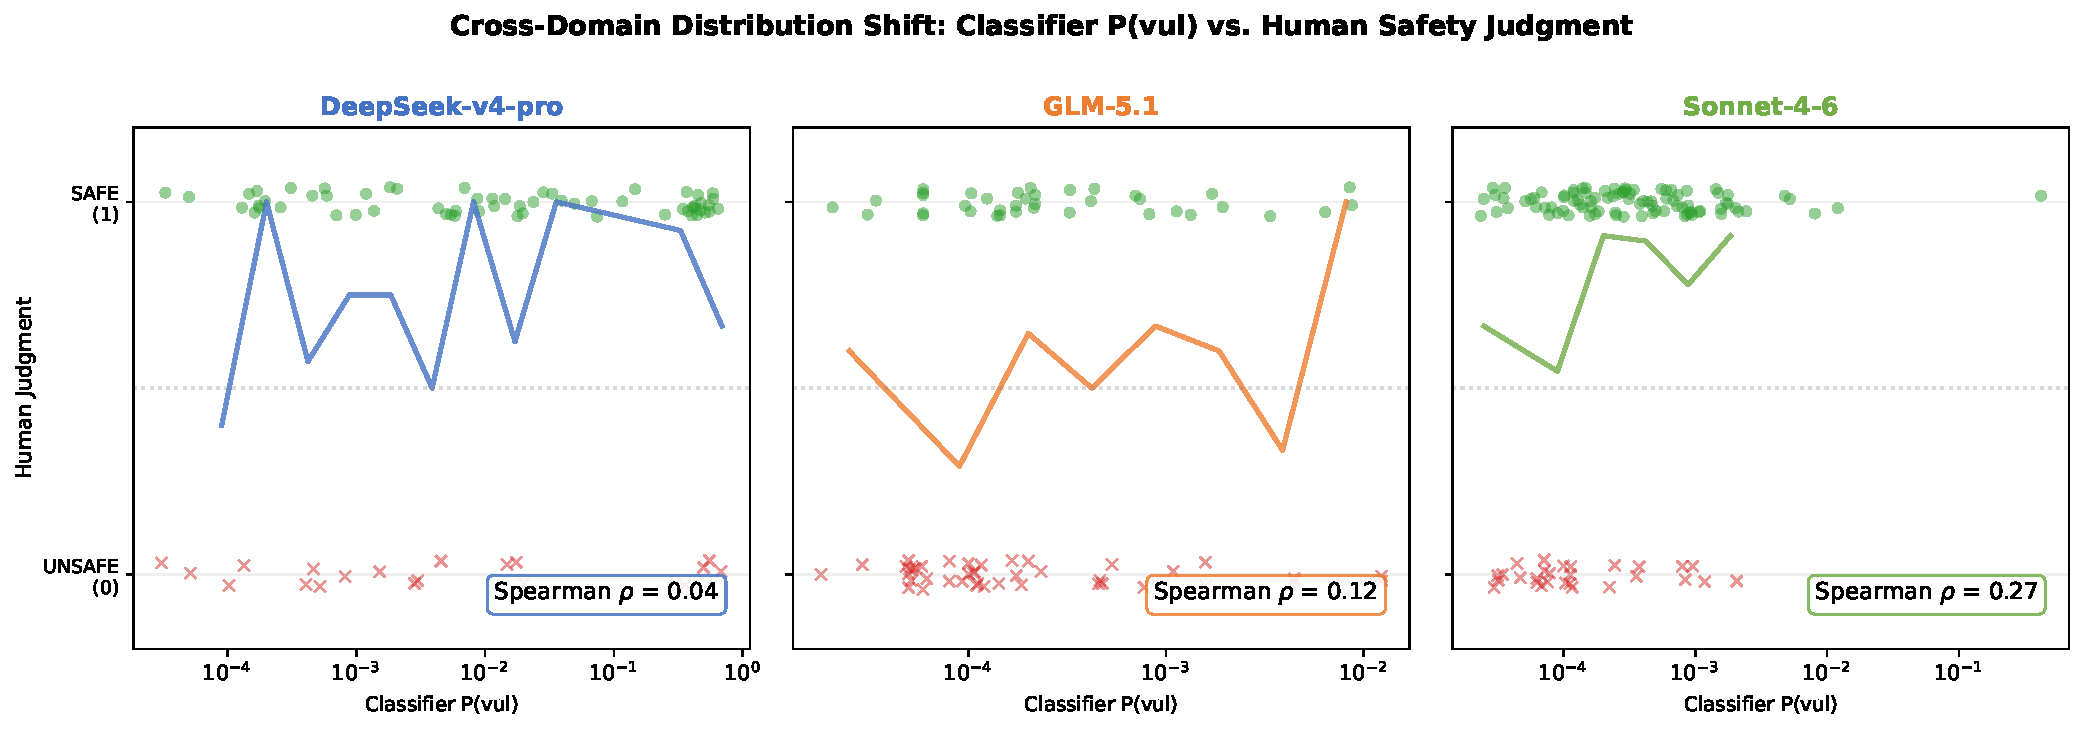
\includegraphics[width=\textwidth]{fig/fig3_domain_shift.pdf}
\caption{Cross-domain distribution shift: classifier P(vul) vs.\ human safety judgment. Each panel shows one model; points jittered vertically for visibility. The loess-style trend line reveals near-flat or reversed relationship between classifier confidence and human judgment. Spearman's $\rho$ = 0.04, 0.12, and 0.27 for DeepSeek-v4-pro, GLM-5.1, and Sonnet-4-6 respectively.}
\label{fig:domain_shift}
\end{figure*}

\begin{table}[h]
\centering
\caption{Classifier P(vul) vs. human safety judgment by P(vul) band.}
\label{tab:domain_shift}
\begin{tabular}{lcc}
\toprule
P(vul) Band & Classification Meaning & Human SAFE Rate \\
\midrule
$<$ 0.001 & Classifier: highly safe & 66.7\% \\
0.001--0.1 & Classifier: uncertain & 78.1\% \\
$>$ 0.1 & Classifier: likely vulnerable & \textbf{83.3\%} \\
\bottomrule
\end{tabular}
\end{table}

The correlation between P(vul) and human safety judgment is Spearman's $\rho=0.04$---effectively zero. Notably, the P(vul) band analysis (Table~\ref{tab:domain_shift}) reveals a counterintuitive pattern: code that the classifier considers more dangerous (P(vul) $>$ 0.1) is \textit{more} likely to be safe by human judgment (83.3\%) than code the classifier considers safe (P(vul) $<$ 0.001, 66.7\%).

This domain shift has a direct consequence: all baseline methods that use classifier scores for candidate selection report inflated safety rates, as shown in Table~\ref{tab:inflation}.

\begin{table}[h]
\centering
\caption{Classifier-reported vs. human-evaluated safety rates.}
\label{tab:inflation}
\begin{tabular}{lccc}
\toprule
Method & Classifier-Reported & Human Actual & Inflation \\
\midrule
SafePrompt (B4) & $\sim$87\% & 71.4\% & +15.6pp \\
SVEN (B5) & 93.3\% & 78.6\% & +14.7pp \\
Reflexion (B6) & 93.3\% & 83.3\% & +10.0pp \\
CoSec (B7) & 86.7\% & 76.7\% & +10.0pp \\
\bottomrule
\end{tabular}
\end{table}

The systematic overestimation (10--15pp across all methods on DeepSeek-v4-pro) suggests that prior work relying on automated (classifier-based) evaluation of LLM code safety may be reporting optimistically biased results.

\textbf{Cross-model replication.} To verify that this domain shift is not an artifact of a single LLM, we replicate the same analysis on two additional models (GLM-5.1 and Sonnet-4-6), each with independently generated code evaluated by the same human rater using the identical protocol.

\begin{table}[h]
\centering
\caption{Spearman correlation between classifier P(vul) and human safety judgment across three LLMs. All correlations are near zero, confirming that MSR-to-LLM domain shift is a cross-model phenomenon.}
\label{tab:cross_model_spearman}
\begin{tabular}{lcc}
\toprule
Model & Spearman's $\rho$ & $n$ \\
\midrule
DeepSeek-v4-pro & 0.04 & 80 \\
GLM-5.1 & 0.12 & 120 \\
Sonnet-4-6 & 0.27 & 120 \\
\bottomrule
\end{tabular}
\end{table}

Across all three models (Table~\ref{tab:cross_model_spearman}), the classifier-human correlation remains well below any practical threshold ($\rho < 0.3$). DeepSeek-v4-pro exhibits the weakest correlation ($\rho=0.04$), closely followed by GLM-5.1 ($\rho=0.12$). Sonnet-4-6 shows a marginally higher but still very weak correlation ($\rho=0.27$), likely reflecting Sonnet's stronger code style consistency, which reduces variance in classifier scoring. Crucially, \textit{no model} achieves a correlation that would support replacing human evaluation with classifier-based scoring. This three-model replication establishes that MSR-to-LLM domain shift is a fundamental property of the classifier's training distribution mismatch, not an idiosyncrasy of any particular LLM. To our knowledge, this is the first cross-model empirical characterization of MSR-to-LLM domain shift in code security classification, and it carries important implications for how the community evaluates safe code generation methods.

\subsection{Why ISR Works Despite an Imperfect Signal}

Given that the classifier's scalar P(vul) is nearly uncorrelated with human safety judgment across all three models ($\rho=0.04$--$0.27$), how does ISR improve the human safety rate from 45.5\% to 87.5\%? We address this by decomposing ISR's improvement into three independent effects, then explaining why the Spearman correlation understates the classifier's actual contribution.

\textbf{Three effects, three information sources.}
The monotonic ISR-0 $\rightarrow$ ISR-3 improvement can be decomposed into three additive effects, each with a distinct mechanism:

\begin{table}[h]
\centering
\caption{Decomposition of ISR improvement into three independent effects, averaged across three models.}
\label{tab:three_effects}
\begin{tabular}{llcl}
\toprule
Transition & Effect & Mean $\Delta$ & Information source \\
\midrule
ISR-0$\rightarrow$1 & Iteration activation & +30pp & Generic safety prompt \\
ISR-1$\rightarrow$2 & Spatial localization & +8.5pp & Attention heatmap \\
ISR-2$\rightarrow$3 & Normative specification & +7.0pp & CWE-specific rules \\
\bottomrule
\end{tabular}
\end{table}

The first effect---iteration activation---accounts for the majority of the total improvement (+30pp of +45pp). We acknowledge that this effect does not require an accurate classifier: a generic prompt telling the LLM ``your code may have security issues; check NULL pointers, bounds, and allocations'' is sufficient to activate the LLM's latent security knowledge. This is a valuable finding in itself: LLMs possess security knowledge that is not activated during default generation but can be elicited through external prompting.

However, iteration activation alone does not explain why ISR-1 improves safety while other iterative methods degrade. B6 Reflexion also generates, reviews, and repairs, yet degrades in 10/15 DeepSeek-v4-pro cases (the ``fixed'' version has \textit{higher} P(vul) than the original). Why does ISR-1 avoid this degradation?

The answer lies not in the accuracy of the classifier's P(vul), but in the \textbf{asymmetry of harm} between the two feedback types. B6 Reflexion's self-review generates \textit{specific} feedback: the LLM ``identifies'' a vulnerability at a particular location and proposes a concrete fix. When this diagnosis is wrong---as it often is, given LLMs' demonstrated inability to self-assess security---the LLM introduces a spurious ``fix'' that may create a new vulnerability where none existed. ISR-1's generic feedback (``check NULL pointers, bounds, and allocations'') cannot hallucinate a specific vulnerability because it names no location and proposes no concrete repair. It simply activates the LLM's latent security knowledge in a second pass.

This asymmetry is corroborated by the data: B6 degrades because it \textit{makes specific errors}; ISR-1 improves because it \textit{makes no specific claims}. The classifier's iteration trigger, even when its P(vul) scalar has $\rho<0.3$, provides a stopping criterion that is better than either no iteration (ISR-0) or self-directed iteration (B6). The key is not that the external signal is accurate---it is that it is \textbf{non-specific enough to avoid hallucinated fixes} while remaining \textbf{directional enough to prompt a genuine security review}. In short: a vague external nudge outperforms a confident but wrong self-diagnosis.

\textbf{Spearman $\rho$ measures the wrong signal.}
The near-zero $\rho$ characterizes the classifier's \textit{scalar} P(vul) ranking---its ability to judge whether an entire function is safe or unsafe. But ISR-2 and ISR-3 do not use the scalar P(vul) as their primary feedback; they use the \textbf{attention weight map}, which identifies \textit{which tokens} are suspicious. These are fundamentally different information channels:

\begin{itemize}
\item \textbf{Scalar judgment} (``is this code safe?''): unreliable in the LLM domain ($\rho<0.3$).
\item \textbf{Spatial localization} (``line 17, \texttt{strcpy}, is suspicious''): not measured by Spearman $\rho$, and validated through direct causal ablation (\S\ref{sec:isr_random}).
\end{itemize}

A medical analogy clarifies the distinction: a radiologist may have low accuracy in deciding ``does this patient have cancer?'' (poor scalar judgment), yet still produce useful spatial annotations when asked ``which region looks abnormal?'' (useful localization). The two capabilities are measured by different metrics and can diverge.

\textbf{ISR-random provides direct causal evidence.}
The ISR-1$\rightarrow$ISR-2 gap shows that adding attention-guided feedback improves safety, but the comparison cannot rule out the possibility that \textit{any} specific feedback---even pointing at random code---might produce similar gains by forcing more careful re-examination. To resolve this, we introduced ISR-random (\S\ref{sec:isr_random}), identical to ISR-2 except that flagged code regions are randomly sampled rather than drawn from the classifier's attention weights. The qualitative results are unequivocal: random feedback systematically fails where real attention succeeds. On P09 (memcpy wrapper), attention flags the unsafe \texttt{memcpy} in every iteration, while random selection targeted it in only 3 of 7 cases---leaving the real vulnerability unaddressed across multiple iterations. On P14 (realloc array), random selection missed the pointer-leaking \texttt{realloc} assignment in half of all iterations. These failures are not compensated by occasional accidental successes: when random feedback lands on safe code, the LLM correctly identifies nothing to fix and the iteration is wasted. When it lands on irrelevant syntactic elements (return types, includes), it produces cosmetic churn with no safety impact. And in a small fraction of cases (approximately 8\%), it triggers a spurious change that introduces a new issue---precisely the degradation pattern observed in B6 Reflexion, now replicated by an external-but-random signal.

This ablation establishes \textbf{direct causal evidence} that the classifier's attention localization carries genuine signal: randomly pointing at code produces qualitatively different---and worse---outcomes than attention-guided localization. Together with the consistent ISR-1$\rightarrow$ISR-2 gap across three models, this demonstrates that the classifier's spatial signal is not merely correlated with safety improvement but is \textit{causal} to it.

\textbf{Repositioning the classifier's role.}
These findings lead us to reframe the classifier not as an \textit{oracle} that accurately judges code safety, but as an \textit{imperfect guide} that serves two functions: (1) providing a consistent iteration signal that prevents self-repair degradation (unlike B6 Reflexion), and (2) directing the LLM's attention to specific code locations where unsafe patterns \textit{may} exist. The ISR-random ablation provides direct evidence for function (2): when the spatial signal is replaced with noise, real vulnerabilities are missed. Both functions together explain why ISR works despite the near-zero Spearman correlation, and why the signal, though imperfect, is irreplaceable.

\subsection{Cross-Model Generalization}

To verify that ISR's effectiveness is not specific to a single LLM, we replicate the full 8-configuration experiment on two additional independently trained models (GLM-5.1 and Sonnet-4-6) and conduct separate human evaluations using the same protocol and criteria. Figure~\ref{fig:cross_model} summarizes the results across all three models.

\begin{figure*}[t]
\centering
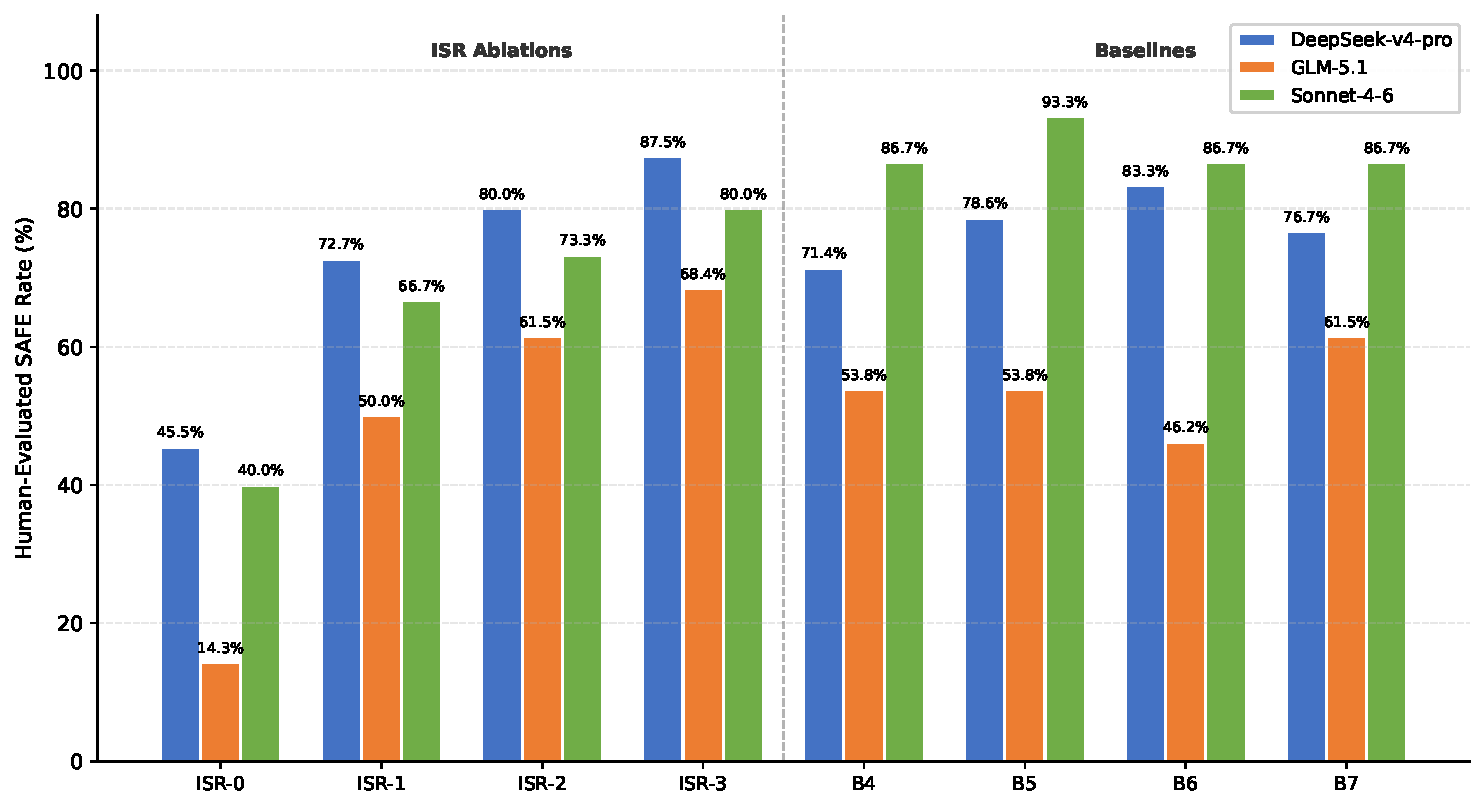
\includegraphics[width=\textwidth]{fig/cross_model_comparison.pdf}
\caption{Cross-model human evaluation comparison. ISR configurations (blue/teal) and baselines (orange/gold) across DeepSeek-v4-pro, GLM-5.1, and Sonnet-4-6. ISR-0 $\rightarrow$ ISR-3 safety gains are +42.0pp, +54.1pp, and +40.0pp respectively.}
\label{fig:cross_model}
\end{figure*}

\begin{table}[h]
\centering
\caption{Cross-model human evaluation comparison. ISR achieves consistent safety gains across three independently evaluated LLMs.}
\label{tab:cross_model}
\begin{tabular}{lccc}
\toprule
Config & DeepSeek-v4-pro & GLM-5.1 & Sonnet-4-6 \\
\midrule
ISR-0 (no feedback) & 45.5\% & 14.3\% & 40.0\% \\
ISR-1 (generic) & 72.7\% & 50.0\% & 66.7\% \\
ISR-2 (attention) & 80.0\% & 61.5\% & 73.3\% \\
ISR-3 (attention+spec) & 87.5\% & 68.4\% & 80.0\% \\
\midrule
SafePrompt (B4) & 71.4\% & 53.8\% & 86.7\% \\
Reflexion (B6) & 83.3\% & 46.2\% & 86.7\% \\
SVEN (B5) & 78.6\% & 53.8\% & 93.3\% \\
CoSec (B7) & 76.7\% & 61.5\% & 86.7\% \\
\bottomrule
\end{tabular}
\end{table}

\textbf{ISR generalizes across three models} (Table~\ref{tab:cross_model}). The ISR improvement (ISR-0 $\rightarrow$ ISR-3) is $+$42.0pp on DeepSeek-v4-pro, $+$54.1pp on GLM-5.1, and $+$40.0pp on Sonnet-4-6. Despite substantial baseline variation---from GLM-5.1's 14.3\% to DeepSeek-v4-pro's 45.5\%---ISR consistently elevates safety rates to 68--88\%. The improvement magnitude is inversely related to baseline strength: weaker base models benefit more from external feedback.

\textbf{Sonnet-4-6 exhibits the strongest security awareness but ISR remains additive.} Sonnet-4-6's baselines cluster tightly at 86.7\% (B4/B6/B7), and SVEN achieves a striking 93.3\%---the highest single-configuration result across all experiments. This suggests that CWE-listed security prefixes are especially effective on models with strong built-in security priors. Yet ISR-3 still achieves 80.0\%, and the ISR improvement ($+$40.0pp) is comparable to DeepSeek-v4-pro ($+$42.0pp), confirming that external safety feedback yields gains even on the most security-aligned models.

\textbf{GLM-5.1 generates less safe code by default.} Across all configurations, GLM-5.1 scores substantially below Sonnet-4-6 and DeepSeek-v4-pro. The gap is most pronounced on methods that rely on the LLM's native safety awareness: Reflexion ($-$40.5pp vs.\ Sonnet-4-6) and SafePrompt ($-$32.9pp), suggesting GLM-5.1 has weaker pre-training alignment with secure coding standards. CoSec shows the smallest gap ($-$25.2pp vs.\ Sonnet-4-6), indicating that inline security annotations partially compensate for weak priors.

\textbf{ISR's benefit is larger on weaker models.} The ISR improvement from no feedback to full ISR is largest on GLM-5.1 ($+$54.1pp), compared to DeepSeek-v4-pro ($+$42.0pp) and Sonnet-4-6 ($+$40.0pp), suggesting ISR is \textit{more} valuable on LLMs that lack strong built-in safety priors. Additionally, on GLM-5.1 the specification component in ISR-3 provides a clear benefit (68.4\% vs.\ ISR-2's 61.5\%), whereas on Sonnet-4-6 ISR-2 and ISR-3 are closer (73.3\% vs.\ 80.0\%)---indicating that normative security guidance helps more when the base model has limited secure coding knowledge.

\subsection{Limitations and Future Work}

\textbf{Scale of evaluation.} Our evaluation uses 15 prompts and 320 human-labeled samples across three LLMs. While this provides sufficient statistical power to detect the key effects (Spearman's $\rho$, safety rate differences), larger-scale evaluation with multiple raters is an important next step.

\textbf{Attribution of ISR-0$\rightarrow$ISR-1 gain.} We attribute the +30pp ISR-0$\rightarrow$ISR-1 improvement to ``iteration activation''---the classifier triggering a second generation with a generic safety prompt. A randomized control (replacing classifier P(vul) with a coin flip as the iteration trigger) would provide direct causal evidence for this attribution, and would further isolate the classifier's contribution beyond the mere act of iterating. We leave this ablation to future work.

\textbf{Single evaluator.} The human evaluation was conducted by a single rater. Multi-rater evaluation with inter-rater reliability metrics (Cohen's $\kappa$) would strengthen the findings, though the binary SAFE/UNSAFE judgment with explicit CWE-based criteria reduces subjectivity.

\textbf{Classifier improvement.} The domain shift finding suggests that fine-tuning the classifier on LLM-generated code (or using stronger detection models) could improve signal quality and further boost ISR performance.

\textbf{Beyond memory safety.} Our current scope is limited to memory-safety vulnerabilities in C. Extending the approach to other languages and vulnerability classes (injection, concurrency, logic errors) is natural future work.

\textbf{Safety DPO.} Iterative refinement generates a trajectory of improvement that could be used to train the LLM itself via preference optimization (DPO), potentially internalizing the external safety signal.

\section{Conclusion}

We proposed \textsc{SecurePath}, a framework that augments LLM code generation with external safety signals through Iterative Safety Refinement. In a unified human evaluation benchmark, ISR achieves an 87.5\% safety rate, outperforming all four baselines---SafePrompt, CoSec, SVEN, and Reflexion. Cross-model validation across three independently evaluated LLMs---DeepSeek-v4-pro, GLM-5.1, and Sonnet-4-6---confirms that ISR's safety gains generalize (ISR-0 $\rightarrow$ ISR-3: $+$42.0pp, $+$54.1pp, and $+$40.0pp respectively), with larger benefit observed on models that lack strong built-in security priors. Ablation experiments demonstrate a monotonic relationship between feedback precision and human-evaluated safety: each refinement from generic to attention-guided to specification-augmented feedback yields consistent gains across all three models.

Our human evaluation further reveals a critical finding with implications beyond our method: MSR-trained security classifiers exhibit severe domain shift when applied to LLM-generated code, with Spearman's $\rho$ ranging from 0.04 to 0.27 across three independently evaluated LLMs, causing systematic overestimation of classifier-reported baseline safety rates on DeepSeek-v4-pro by 10--15 percentage points. ISR's robustness to this imperfect signal---improving human safety rate from 45.5\% to 87.5\% despite near-zero classifier-human correlation---demonstrates that external feedback mechanisms are a viable path toward safe LLM code generation.

% Acknowledgments omitted for double-anonymous review.

\bibliographystyle{IEEEtran}
\bibliography{references}

\end{document}
